Weak gravitational lensing (WL), also known as cosmic shear, refers to the subtle distortions in the images of distant source caused by the gravitational fields of intervening mass distributions. Unlike strong lensing, which produces noticeable effects such as multiple images or arcs, weak lensing induces small, coherent distortions that require statistical analysis to detect and interpret. For the standard approach to lensing, we refer to \citet{1992grle.book.....S}, \citet{2001PhR...340..291B} and \citet{2010CQGra..27w3001B}.

\section{Lens Equation}
\subsection{Derivation}
To derive the lens equation, we consider a perturbed FLRW metric, which incorporates gravitational potential perturbations. The metric is expressed as
\begin{equation}
    ds^2 = -\left(1 + \frac{2\Phi}{c^2}\right)c^2 dt^2 + a^2(t) \left(1 - \frac{2\Psi}{c^2}\right) \left[ d\chi^2 + f_K^2(\chi) \, \omega_{ab} \, dx^a dx^b \right] \quad (a, b = 2, 3),
    \label{eq:perturbed_metric}
\end{equation}
where the angular part of the metric is defined by
\begin{equation}
    \omega_{ab} \, dx^a dx^b := d\theta^2 + \sin^2 \theta \, d\phi^2.
    \label{eq:angular_metric}
\end{equation}
In this context, \( \Phi \) and \( \Psi \) represent the scalar gravitational potentials, and \( f_K(\chi) \) encodes the spatial curvature as previously defined in Eq.~\eqref{eq:fk_definition}.

The trajectory of light within this spacetime is governed by the geodesic equation, which is given by
\begin{equation}
    \frac{d^2 x^\mu}{d\lambda^2} + \Gamma^\mu_{\alpha \beta} \frac{dx^\alpha}{d\lambda} \frac{dx^\beta}{d\lambda} = 0,
    \label{eq:geodesic_equation}
\end{equation}
where \( \lambda \) is an affine parameter and \( \Gamma^\mu_{\alpha \beta} \) are the Christoffel symbols corresponding to the metric in Equation~\eqref{eq:perturbed_metric}.

To facilitate the derivation, we reparametrize the geodesic equation by substituting the affine parameter \( \lambda \) with the comoving radial distance \( \chi \). Applying the chain rule, the geodesic equation transforms to
\begin{equation}
    \frac{d^2 x^\mu}{d\chi^2} + \Gamma^\mu_{\alpha \beta} \frac{dx^\alpha}{d\chi} \frac{dx^\beta}{d\chi} - \frac{d^2 \lambda}{d\chi^2} \left( \frac{d\lambda}{d\chi} \right)^{-1} \frac{dx^\mu}{d\chi} = 0.
    \label{eq:geodesic_reparametrized}
\end{equation}

Setting \( \mu = 1 \) (where \( x^1 = \chi \)) in Equation~\eqref{eq:geodesic_reparametrized} and simplifying, we obtain
\begin{equation}
    \frac{d^2 x^\mu}{d\chi^2} + \left( \Gamma^\mu_{\alpha \beta} - \Gamma^1_{\alpha \beta} \right) \frac{dx^\alpha}{d\chi} \frac{dx^\beta}{d\chi} = 0.
    \label{eq:geodesic_mu1}
\end{equation}

The evaluation of Equation~\eqref{eq:geodesic_mu1} requires the computation of the Christoffel symbols. Additionally, the derivative \( c \, dt / d\chi \) is derived from the null condition
\begin{equation}
    g_{\mu \nu} \frac{dx^\mu}{d\chi} \frac{dx^\nu}{d\chi} = 0,
    \label{eq:null_condition}
\end{equation}
yielding
\begin{equation}
    \frac{c \, dt}{d\chi} = -a(t) \left[ 1 - \frac{\Phi}{c^2} - \frac{\Psi}{c^2} + \frac{f_K^2(\chi)}{2} \omega_{ab} \frac{dx^a}{d\chi} \frac{dx^b}{d\chi} \right],
    \label{eq:dt_dchi}
\end{equation}
valid to first order in \( \Phi \) and second order in \( dx^a / d\chi \). Notably, for the evaluation of Equation~\eqref{eq:geodesic_mu1}, only the zeroth-order term \( c \, dt / d\chi = -a(t) \) is required. However, the inclusion of perturbative terms in Equation~\eqref{eq:dt_dchi} is essential for subsequent derivations of the lens equation.

Focusing on the angular components (\( \mu = a \)) of Equation~\eqref{eq:geodesic_mu1}, we derive the following differential equation:
\begin{equation}
    \frac{d^2 x^a}{d\chi^2} + 2 \frac{f_K'(\chi)}{f_K(\chi)} \frac{dx^a}{d\chi} + \omega^{ab} \frac{\Phi_b + \Psi_b}{c^2 f_K^2(\chi)} = 0,
    \label{eq:geodesic_angular}
\end{equation}
where \( \Phi_b \) and \( \Psi_b \) denote the derivatives of the gravitational potentials with respect to the angular coordinates \( x^a \).
Integrating Equation~\eqref{eq:geodesic_angular} twice with respect to \( \chi \), we obtain
\begin{eqnarray}
    x^a(\chi_s) - x^a(0) &=& -\frac{1}{c^2} \int_0^{\chi_s} d\chi' \int_0^{\chi'} d\chi \, \omega_{ab} \left[ \Phi_b(\chi, \theta(\chi)) + \Psi_b(\chi, \theta(\chi)) \right] \nonumber \\
    &=& -\frac{1}{c^2} \int_0^{\chi_s} d\chi \, \omega_{ab} \left[ \Phi_b(\chi, \theta(\chi)) + \Psi_b(\chi, \theta(\chi)) \right] \int_{\chi}^{\chi_s} d\chi' \frac{1}{f_K^2(\chi')} \nonumber \\
    &=& -\frac{1}{c^2} \int_0^{\chi_s} d\chi \, \omega_{ab} \left[ \Phi_b(\chi, \theta(\chi)) + \Psi_b(\chi, \theta(\chi)) \right] \frac{f_K(\chi_s - \chi)}{f_K(\chi_s)f_K(\chi)},
    \label{eq:xa_integrated}
\end{eqnarray}
where \( \chi_s \) denotes the comoving radial distance to the source, and \( x^a(0) \) is the angular position at the observer's location.
Defining $(\nabla_\theta)^a = \omega^{ab} \partial_b$, the angular position of the source galaxy $\boldsymbol{\beta}$ is related to the observed angular position $\boldsymbol{\theta}$ by
\begin{equation}
    \boldsymbol{\theta}(\chi_s) = \boldsymbol{\theta}(0) - \frac{1}{c^2} \int_0^{\chi_s} d\chi \, \nabla_\theta \left[ \Phi\left(\chi, \boldsymbol{\theta}(\chi)\right) + \Psi\left(\chi, \boldsymbol{\theta}(\chi)\right) \right] \frac{f_K(\chi_s - \chi)}{f_K(\chi_s)f_K(\chi)}.
    \label{eq:lens_equation}
\end{equation}
Applying the Born approximation \citep{1926ZPhy...38..803B}, and assume that $\Phi = \Psi$, we can simplify the lens equation to:
\begin{equation}
    \boldsymbol{\theta}(\chi_s) = \boldsymbol{\theta}(0) - \frac{2}{c^2} \int_0^{\chi_s} d\chi \, \nabla_\theta \left[ \Phi\left(\chi, \boldsymbol{\theta}(0)\right) \right]\frac{f_K(\chi_s - \chi)}{f_K(\chi_s)f_K(\chi)}.
    \label{eq:lens_equation_born}
\end{equation}
This final expression constitutes the lens equation, encapsulating the deflection of light due to the gravitational potentials \( \Phi \) and \( \Psi \) along the line of sight. 

\subsection{Lensing Matrix}
\begin{figure}[ht]
    \centering
    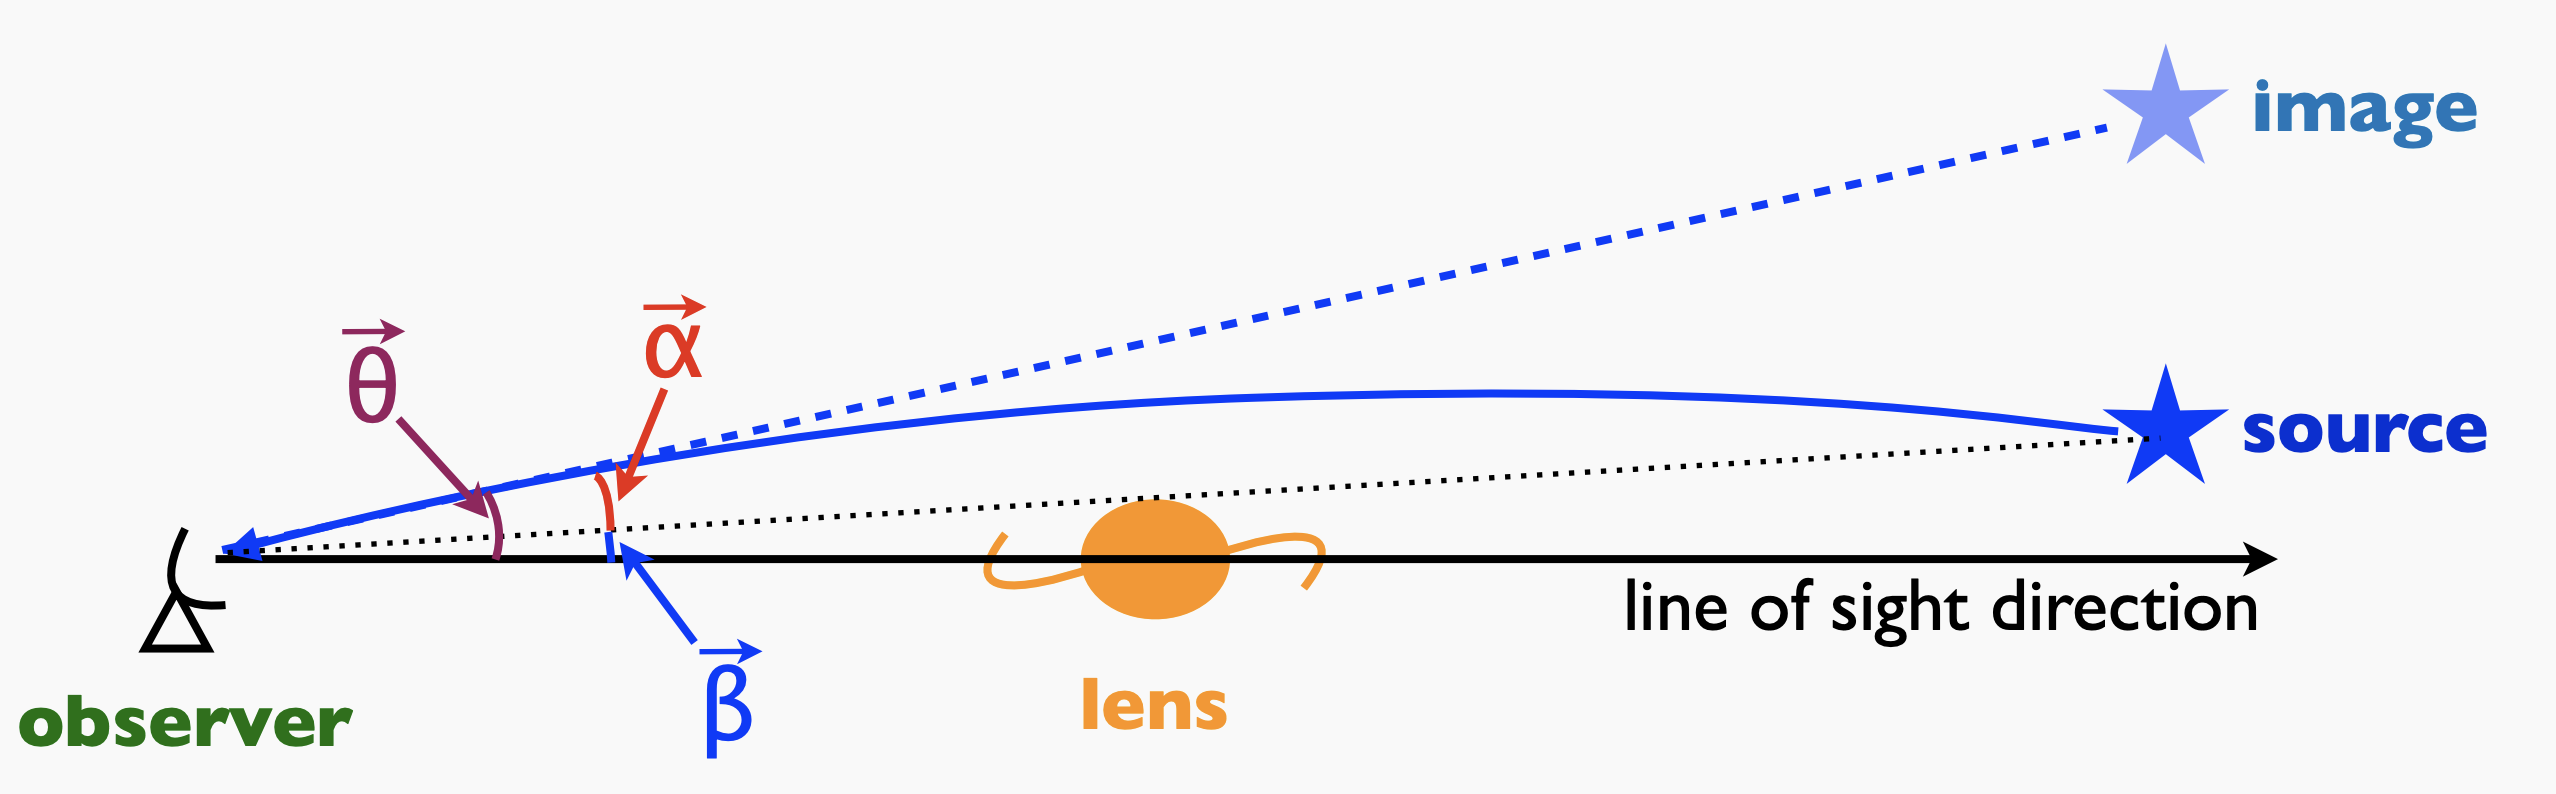
\includegraphics[width=\textwidth]{figures/Lens_overview_Oguri.png}
    \caption[Schematic representation of the lensing geometry]{Schematic representation of the lensing geometry. The source is located at $\boldsymbol{\beta}$, while the observed image is at $\boldsymbol{\theta}$. The deflection angle $\boldsymbol{\alpha}$ is the difference between the observed and true angular positions.}
    \label{fig:lens_geometry}
\end{figure}
Redefining the notation in Eq.~\eqref{eq:lens_equation_born} and considering the angular position of the source $\boldsymbol{\beta} = \boldsymbol{\theta}(\chi_s)$ and the observed angular position $\boldsymbol{\theta} = \boldsymbol{\theta}(0)$ (see Fig.~\ref{fig:lens_geometry}), we can express the lens equation as \citep{2001PhR...340..291B, 2009A&A...499...31H, 2015RPPh...78h6901K}:
\begin{equation}
    \boldsymbol{\beta} = \boldsymbol{\theta} - \boldsymbol{\alpha}(\boldsymbol{\theta}),
    \label{eq:lens_equation_vector}
\end{equation}
where the deflection angle \( \boldsymbol{\alpha}(\boldsymbol{\theta}) \) is defined by:
\begin{equation}
    \boldsymbol{\alpha}(\boldsymbol{\theta}) = \nabla_{\boldsymbol{\theta}} \psi(\boldsymbol{\theta}), \quad \psi(\boldsymbol{\theta}) = \frac{2}{c^2} \int_0^{\chi_s} d\chi \, \frac{f_K(\chi_s - \chi)}{f_K(\chi_s)f_K(\chi)} \Phi\left(f_K(\chi) \boldsymbol{\theta}, \chi\right).
    \label{eq:deflection_angle}
\end{equation}
The mapping between the source plane and the image plane can be described by the Jacobian matrix $\mathcal{A}$, which relates infinitesimal displacements in the source position to displacements in the image position:
\begin{equation}
\label{eq:jacobian_matrix}
    \mathcal{A} := \frac{\partial \boldsymbol{\beta}}{\partial \boldsymbol{\theta}} = 
    \begin{pmatrix}
        1 - \kappa - \gamma_1 & -\gamma_2 \\
        -\gamma_2 & 1 - \kappa + \gamma_1
    \end{pmatrix}
    = \left(1 - \kappa \right) 
    \begin{pmatrix}
        1 & 0 \\
        0 & 1
    \end{pmatrix}
    - |\gamma|
    \begin{pmatrix}
        \cos{2\phi} & \sin{2\phi} \\
        \sin{2\phi} & -\cos{2\phi}
    \end{pmatrix},
\end{equation}
where $\kappa$ is the convergence and $\gamma = \gamma_1 + i\gamma_2 = |\gamma| e^{2i\phi}$ is the shear.
The quantities $\kappa$ and $\gamma$ will be discussed in detail in the subsequent sections.
Figure~\ref{fig:distortion} illustrates the effects of gravitational lensing on the shapes of background sources through the lensing matrix $\mathcal{A}$. The panels demonstrate how the combined effects of convergence and shear components in the Jacobian matrix $\mathcal{A}$ lead to complex distortions of background sources.
\begin{figure}[ht]
    \centering
    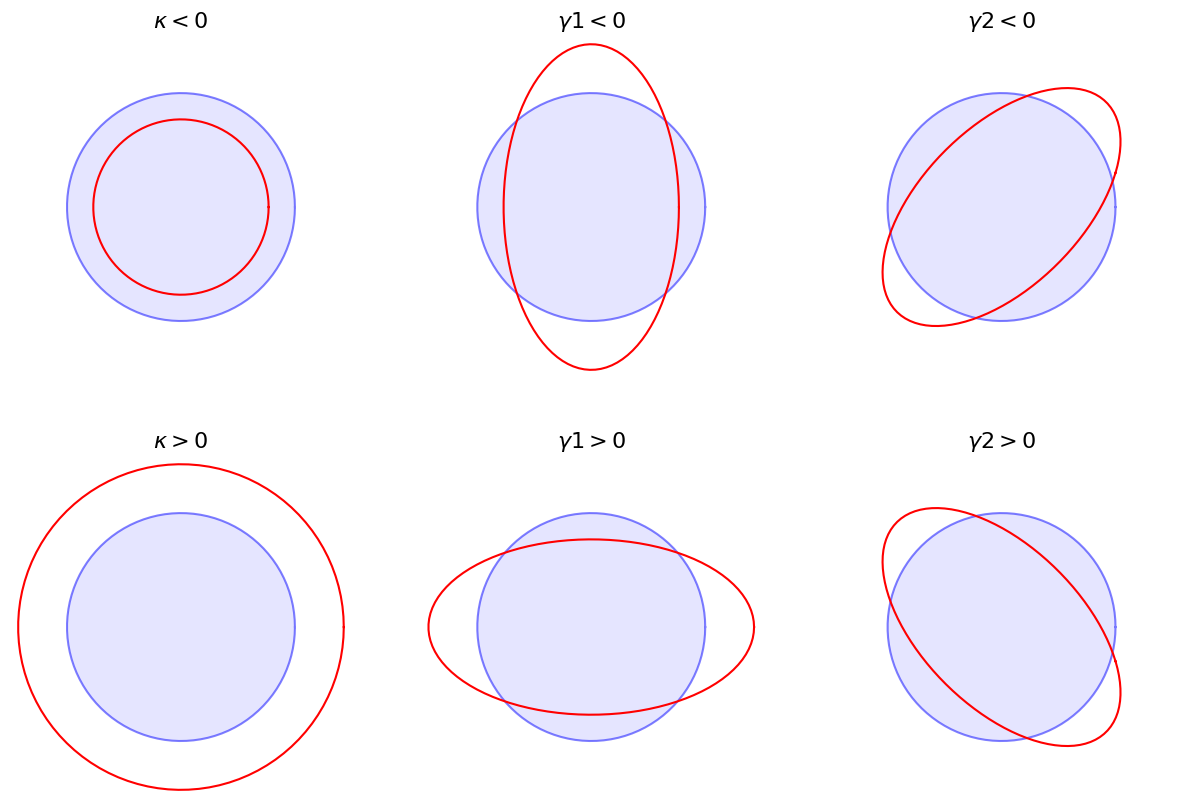
\includegraphics[width=0.8\textwidth]{figures/distortion.png}
    \caption[Illustration of Gravitational Lensing]{Illustration of the distortion of background sources due to gravitational lensing. The left panel depict the effect of the convergence $\kappa$ and the middle and right panels show the components of the shear $\gamma = \gamma_1 + i\gamma_2$ on circular background sources. Positive and negative values of $\kappa$ cause isotropic magnification or demagnification, while $\gamma_1$ and $\gamma_2$ introduce anisotropic distortions, stretching the sources along or at an angle to the principal axes.}
    \label{fig:distortion}
\end{figure}

\section{Convergence} \label{sec:convergence}
\subsection{Definition}
From the lensing matrix in Eq.~\eqref{eq:jacobian_matrix}, the convergence $\kappa$ is defined as:
\begin{equation}
    \label{eq:convergence}
        \kappa(\boldsymbol{\theta}) := \frac{1}{2} \left( \frac{\partial^2 \psi}{\partial \theta_1^2} + \frac{\partial^2 \psi}{\partial \theta_2^2} \right) = \frac{1}{2} \nabla_{\boldsymbol{\theta}}^2 \psi(\boldsymbol{\theta})
\end{equation}
with $\theta_1$ and $\theta_2$ representing the angular coordinates on the sky.
In Fourier space, the convergence field could be expressed as:
\begin{equation}
    \label{eq:fourier_convergence}
    \tilde{\kappa}(\boldsymbol{\ell}) = \int d^2\theta \, e^{-i\boldsymbol{\ell} \cdot \boldsymbol{\theta}} \kappa(\boldsymbol{\theta}) = \frac{1}{2} \ell^2 \tilde{\psi}(\boldsymbol{\ell}),
\end{equation}
where $\tilde{(\quad)}$ denotes the Fourier transform of the corresponding quantity and $\ell = |\boldsymbol{\ell}|$ is the Fourier counterpart to the angular position $\boldsymbol{\theta}$.
\subsection{Convergence from Density Contrast}
In a flat universe, the Poisson equation in comoving coordinates is expressed as
\begin{align}
\label{eq:poisson_flat}
    \nabla_{\mathbf{x}}^2 \Phi(\mathbf{x}, \chi) &= 4\pi G a^2(\chi) \bar{\rho}_m(\chi) \delta(\mathbf{x}, \chi) \nonumber\\ 
    &= 4\pi G a^2(\chi) \left[ \frac{3 H_0^2 \Omega_m}{8 \pi G} a^{-3}(\chi) \right] \delta(\mathbf{x}, \chi) \nonumber \\ 
    &= \frac{3}{2} \Omega_m H_0^2 a^{-1}(\chi) \delta(\mathbf{x}, \chi),
\end{align}
where we utilized Eq.~\eqref{eq:friedmann_rewritten} and Eq.~\eqref{eq:critical_density}.
Substituting the expression for $\Phi$ from Eq.~\eqref{eq:poisson_flat} into the lensing potential (Eq.~\eqref{eq:deflection_angle}) and subsequently into the convergence (Eq.~\eqref{eq:convergence}), we derive:
\begin{eqnarray}
    \label{eq:convergence_integral}
    \kappa(\boldsymbol{\theta}) 
    &=& \frac{1}{c^2} \int_0^{\chi_s} \mathrm{d}\chi \, \frac{f_K(\chi_s - \chi)}{f_K(\chi_s) f_K(\chi)} \left[ \frac{1}{f_K^2(\chi)} \nabla_{\mathbf{x}}^2 \Phi\left(\mathbf{x}, \chi\right) \right] \nonumber \\
    &=& \int_0^{\chi_s} \mathrm{d}\chi \, \frac{3 \Omega_m H_0^2}{2 c^2} \, \frac{f_K(\chi_s - \chi) f_K(\chi)}{f_K(\chi_s)} \frac{a^{-1}(\chi)}{f_K^3(\chi)} \delta\left(\mathbf{x}, \chi\right) \nonumber \\
    &=& \int_0^{\chi_s} \mathrm{d}\chi \, W(\chi, \chi_s) \, \delta\left(\mathbf{x}, \chi\right),
\end{eqnarray}
where the lensing efficiency function $W(\chi, \chi_s)$ is defined by:
\begin{equation}
    \label{eq:lensing_efficiency}
    W(\chi, \chi_s) := \frac{3 \Omega_m H_0^2}{2 c^2} \frac{f_K(\chi) f_K(\chi_s - \chi)}{f_K(\chi_s)} \frac{a^{-1}(\chi)}{f_K^2(\chi)}.
\end{equation}
In a flat universe ($f_K(\chi) = \chi$), this simplifies to:
\begin{equation}
    \label{eq:lensing_efficiency_flat}
    W(\chi, \chi_s) = \frac{3 \Omega_m H_0^2}{2 c^2} a^{-1}(\chi) \frac{\chi (\chi_s - \chi)}{\chi_s}.
\end{equation}

\section{Shear}
The shear $\gamma$ encapsulates the anisotropic stretching of galaxy images induced by gravitational lensing. Unlike convergence, which affects the size and brightness of images isotropically, shear induces distortions that alter the shapes of background galaxies coherently. 
\subsection{Definition}
The shear components $\gamma_1$ and $\gamma_2$ describe distortions along different axes and are related to the lensing potential $\psi$ by:
\begin{equation}
    \label{eq:physical_shear}
    \gamma_1 := \frac{1}{2} \left( \frac{\partial^2 \psi}{\partial \theta_1^2} - \frac{\partial^2 \psi}{\partial \theta_2^2} \right), \quad \gamma_2 := \frac{\partial^2 \psi}{\partial \theta_1 \partial \theta_2}.
\end{equation}
In Fourier space, the shear field can be expressed as:
\begin{equation}
    \label{eq:fourier_shear}
    \tilde{\gamma_1}(\boldsymbol{\ell}) = \tfrac{1}{2} \left( \ell_1^2 - \ell_2^2 \right) \tilde{\psi}(\boldsymbol{\ell}) \quad
    \tilde{\gamma_2}(\boldsymbol{\ell}) = \ell_1 \ell_2 \tilde{\psi}(\boldsymbol{\ell}) ,
\end{equation}
where $\tilde{\gamma_1}(\boldsymbol{\ell})$ and $\tilde{\gamma_2}(\boldsymbol{\ell})$ are the Fourier transforms of $\gamma_1(\boldsymbol{\theta})$ and $\gamma_2(\boldsymbol{\theta})$, respectively. 
Similar as Eq.~\eqref{eq:jacobian_matrix}, the shear field can be expressed in complex form as:
\begin{equation}
    \label{eq:fourier_shear1}
    \tilde{\gamma}(\boldsymbol{\ell}) := \tilde{\gamma}_1 + i\tilde{\gamma}_2 = |\tilde{\gamma}(\boldsymbol{\ell})|e^{2i\phi_\ell}, \quad \tan (2\phi_\ell) = \tilde{\gamma}_2 / \tilde{\gamma}_1.
\end{equation}
Therefore, the shear field in Fourier space is directly related to the convergence field combining Eq.\eqref{eq:fourier_convergence} and Eq.\eqref{eq:fourier_shear} \citep{1993ApJ...404..441K}:
\begin{equation}
    \tilde{\kappa}(\boldsymbol{\ell}) = \frac{\ell_1^2 - \ell_2^2 + 2i\ell_1\ell_2}{\ell^2} \tilde{\gamma}(\boldsymbol{\ell}).
    \label{eq:kappa_gamma_relation}
\end{equation}
\subsection{E-mode and B-mode}
The shear field can be decomposed into two distinct modes: the \textbf{E-mode} (gradient component) and the \textbf{B-mode} (curl component). 
By rotating the complex shear field to align with the principal axes of the shear $\tilde{\gamma}_{EB} = e^{-2i\phi_l} \tilde{\gamma}$, we can express the shear field in terms of the E-mode and B-mode components:
\begin{equation}
    \begin{pmatrix}
        \tilde{\gamma}_E \\
        \tilde{\gamma}_B
        \end{pmatrix}
        :=
        \begin{pmatrix}
        \cos 2\phi_l & \sin 2\phi_l \\
        -\sin 2\phi_l & \cos 2\phi_l
        \end{pmatrix}
        \begin{pmatrix}
        \tilde{\gamma}_1 \\
        \tilde{\gamma}_2
    \end{pmatrix}
    \label{eq:EB_decomposition}
\end{equation}
where $\tilde{\gamma}_E$ and $\tilde{\gamma}_B$ are the E-mode and B-mode components of the shear, respectively. The E-mode represents the gradient component of the shear field, while the B-mode describes the curl component.

For standard gravitational lensing by density fluctuations, the B-mode component $\tilde{\gamma}_B(\boldsymbol{\ell})$ is expected to vanish in the absence of systematics or additional physical effects. This implies that all the shear signal is contained within the E-mode.such that:
\begin{equation}
    \tilde{\gamma}_E(\boldsymbol{\ell}) = \tilde{\kappa}(\boldsymbol{\ell}), \quad \tilde{\gamma}_B(\boldsymbol{\ell}) = 0.
    \label{eq:EB_decomposition_standard}
\end{equation}

\section{Estimation of Lensing Fields}
In the case of cosmic shear, not the convergence but the shear is measured from the observed galaxy shapes. Theoretical predictions of the convergence can be related to the observed shear using the relationship in Eq.~\eqref{eq:kappa_gamma_relation}. 
Here, we introduce a concept of the reduced shear. Furthermore, a convergence field can be estimated from the observed galaxy shapes \citep{1993ApJ...404..441K} and can be estimated from magnification \citep{2001PhR...340..291B}.

\subsection{Ellipticity and Reduced Shear}
To quantify the shapes of galaxies, we use the second moments of their surface brightness distributions $I(\theta)$. For each galaxy, the second moments $Q_{ab}$ are defined as \citep{2001PhR...340..291B}:
\begin{equation}
    Q_{ab} := \frac{\int d^2\theta\, I(\theta) \theta_a \theta_b}{\int d^2\theta\, I(\theta)},
    \label{eq:second_moments}
\end{equation}
where $\theta = (\theta_1, \theta_2)$ is the angular position relative to the galaxy center. The complex ellipticity $\epsilon$ of the galaxy is then defined as:
\begin{equation}
    \epsilon := \frac{Q_{11} - Q_{22} + 2i Q_{12}}{Q_{11} + Q_{22}}.
    \label{eq:complex_ellipticity}
\end{equation}

Gravitational lensing transforms the image of a source galaxy via the Jacobian matrix $A$ (see Eq.~\eqref{eq:jacobian_matrix}). Assuming that the surface brightness is conserved during lensing, $I^{(s)}(\beta) = I(\theta)$, the second moments in the source plane $Q_{ab}^{(s)}$ are related to those in the image plane by:
\begin{equation}
    Q_{ab}^{(s)} = \frac{\int d^2\beta\, I^{(s)}(\beta) \beta_a \beta_b}{\int d^2\beta\, I^{(s)}(\beta)} \approx A_{ac} A_{bd} Q_{cd},
    \label{eq:second_moments_source}
\end{equation}
where we have approximated the size of the galaxy as sufficiently small so that the lensing distortion is constant across the galaxy image.

By expanding the components of $Q_{ab}^{(s)}$ and performing straightforward calculations (see \citealt{1992grle.book.....S} for details), we find that the intrinsic ellipticity $\epsilon^{(s)}$ is related to the observed ellipticity $\epsilon$ through:
\begin{equation}
    \epsilon^{(s)} = \frac{(1 - \kappa)^2 \epsilon - 2 (1 - \kappa) \gamma + \gamma^2 \epsilon^*}{(1 - \kappa)^2 + |\gamma|^2 - 2 (1 - \kappa) \text{Re}[\gamma \epsilon^*]},
    \label{eq:reduced_shear_ellipticity}
\end{equation}
where $\epsilon^*$ denotes the complex conjugate of $\epsilon$, and $\text{Re}$ denotes the real part.

Introducing the \emph{reduced shear} $g = \gamma / (1 - \kappa)$, the above equation simplifies to \citep{1995A&A...294..411S}:
\begin{equation}
    \epsilon^{(s)} = \frac{\epsilon - 2g + g^2 \epsilon^*}{1 + |g|^2 - 2 \text{Re}[g \epsilon^*]}.
    \label{eq:reduced_shear_ellipticity_g}
\end{equation}
This relation indicates that weak lensing measurements are sensitive to the reduced shear $g$ rather than the shear $\gamma$ directly. In the weak lensing regime, where $|\kappa|, |\gamma| \ll 1$, and assuming that the intrinsic ellipticities of galaxies are randomly oriented (i.e., $\langle \epsilon^{(s)} \rangle = 0$), the observed ellipticity becomes an unbiased estimator of the reduced shear:
\begin{equation}
    \langle \epsilon \rangle \approx g \approx \gamma.
    \label{eq:reduced_shear_expectation}
\end{equation}
However, in the weak-lensing regime, the shear cannot be detected from an individual galaxy due to the dominance of intrinsic shape noise. The typical root mean square (rms) of the intrinsic ellipticity is $\sigma_\epsilon \approx 0.26$ \citep{2019A&A...627A..59E}, which necessitates averaging over a large number of galaxies to measure the shear signal accurately.
The noise for the reduced shear estimator is dominated by Poisson noise, which is given by:
\begin{equation}
    \sigma_\gamma = \frac{\sigma_\epsilon}{\sqrt{N}},
    \label{eq:reduced_shear_noise}
\end{equation}
where $N$ is the number of galaxies used in the shear estimation. It is known that the following transformation of convergence does not change the reduced shear, 
\begin{equation}
    \kappa' = \lambda \kappa + (1 - \lambda),
    \label{eq:kappa_transformation}
\end{equation}
where $\lambda$ is a arbitary constant. This degree of freedom in the convergence
field is known as the mass-sheet degeneracy \citep{1985ApJ...289L...1F}.

\subsection{From Shear to Convergence}
As we have seen in Eq.~\eqref{eq:kappa_gamma_relation}, shear and convergence are related through the Fourier transform. Following \citet{1993ApJ...404..441K}, the relation between the shear and convergence fields in real space can be expressed as:
\begin{equation}
    \gamma(\boldsymbol{\theta}) = \frac{1}{\pi} \int d^2\theta' \, \mathcal{D}(\boldsymbol{\theta} - \boldsymbol{\theta'}) \kappa(\boldsymbol{\theta'}),
\end{equation}
where $\mathcal{D}(\boldsymbol{\theta})$ is a kernel function defined by:
\begin{equation}
    \mathcal{D}(\boldsymbol{\theta}) = - \frac{\theta_1^2 - \theta_2^2 + 2i\theta_1\theta_2}{\boldsymbol{\theta}^4} = - \frac{1}{(\theta_1 - i\theta_2)^2}.
\end{equation}
Therefore, the convolution with the kernel function in Fourier space yields:
\begin{equation}
    \tilde{\gamma}(\boldsymbol{\ell}) = \frac{1}{\pi}\tilde{\mathcal{D}}(\boldsymbol{\ell}) \tilde{\kappa}(\boldsymbol{\ell}),
\end{equation}
The Fourier transform of the kernel function,  $\tilde{\mathcal{D}}(\boldsymbol{\ell})$, is given by:
\begin{equation}
    \tilde{\mathcal{D}}(\boldsymbol{\ell}) = \pi \frac{\ell_1^2 - \ell_2^2 + 2i\ell_1\ell_2}{\ell^2} 
\end{equation}
It is notable that this kernel function and its conjugate satisfies:
\begin{equation}
    \tilde{\mathcal{D}}(\boldsymbol{\ell})\tilde{\mathcal{D}}^*(\boldsymbol{\ell}) = \pi^2 \left(\frac{\ell_1^2 - \ell_2^2 + 2i\ell_1\ell_2}{\ell^2}\right)\left(\frac{\ell_1^2 - \ell_2^2 - 2i\ell_1\ell_2}{\ell^2}\right) = \pi^2.
\end{equation}
Substituting the expression for $\tilde{\mathcal{D}}(\boldsymbol{\ell})$ into the relation between the shear and convergence fields, we find:
\begin{equation}
    \tilde{\kappa}(\boldsymbol{\ell}) = \frac{1}{\pi}\tilde{\gamma}(\boldsymbol{\ell}) \tilde{\mathcal{D}}^*(\boldsymbol{\ell}).
\end{equation}
\begin{equation}
    \kappa(\boldsymbol{\theta}) = \kappa_0 + \frac{1}{\pi} \int d^2\theta' \, \mathcal{D}^*(\boldsymbol{\theta} - \boldsymbol{\theta'}) \gamma(\boldsymbol{\theta'}).
\end{equation}
The constant term $\kappa_0$ arises from the unknown $\ell = 0$ mode in the Fourier space, which is not constrained by the observed shear field.

\begin{comment}
\section{Magnification}
\textbf{Magnification} $\mu$ quantifies the change in the apparent size and brightness of background sources due to lensing. It is related to convergence and shear through the determinant of the lensing Jacobian matrix $\mathcal{A}$:
\begin{equation}
    \mu := \frac{1}{\det(\mathcal{A})} = \frac{1}{(1 - \kappa)^2 - |\gamma|^2}.
    \label{eq:magnification}
\end{equation}
Under the weak lensing approximation ($\kappa, |\gamma| \ll 1$), the magnification simplifies to:
\begin{equation}
    \mu \approx 1 + 2\kappa.
    \label{eq:magnification_weak}
\end{equation}
\subsection{Magnification Bias}
\textbf{Magnification bias} arises from the interplay between magnification and the intrinsic properties of the background source population. Specifically, it refers to the change in the observed number density of background sources due to lensing-induced magnification.
The effect of magnification bias on the observed number density $n_{\text{obs}}$ of background sources is given by \citep{2001PhR...340..291B}:
\begin{equation}
    n_{\text{obs}}(>F, z) = \frac{1}{\mu(\theta, z)} n_0\left(>\frac{F}{\mu(\theta, z)}, z\right),
    \label{eq:magnification_bias}
\end{equation}
where $n(>F, z)$ denotes the number density of sources with flux greater than $F$ at redshift $z$.

Under the weak lensing approximation, the change in the observed number density due to magnification bias can be expressed as:
\begin{equation}
    \frac{\Delta n_{\text{obs}}}{n_{\text{obs}}} = 2 (\alpha - 1) \kappa,
    \label{eq:magnification_bias_weak}
\end{equation}
where $\alpha$ is the logarithmic slope of the source number counts.
It indicates that the observed number density of background sources is enhanced (suppressed) in regions of positive (negative) convergence.
\end{comment}